\paragraph{La classe BDD}


\begin{minipage}
    {\linewidth}
    \centering
    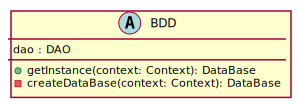
\includegraphics[width=0.30\linewidth]{../schemas/Conception_detaillee/classe_bdd.pdf}
    \captionof{figure}{Diagramme de classe de BDD}
\end{minipage}
\subparagraph{Philosophie de conception \newline} 

\medspace

La classe BDD a pour rôle d'instancier l'interface DAO.  

\subparagraph{Description structurelle \newline}

\medspace

\textbf{Attributs :}

\begin{itemize}
    \item \textbf{dao : DAO} --- Opération qui permet d'instancier l'interface DAO. 
    \item \textbf{getInstance(context: Context): DataBase} --- Opération qui de créer une instance de la base de données.
    \item \textbf{createDataBase(context: Context): DataBase} --- Opération qui de créer la base de données. 
\end{itemize}

\textbf{Services offerts :}

N.A.

